\documentclass[a4paper]{article}


\usepackage[utf8]{inputenc}
\usepackage[T1]{fontenc}
\usepackage{textcomp}
\usepackage{mathtools,amssymb,amsthm}
\usepackage{lmodern}
\usepackage{geometry}
\geometry{hmargin=1cm,vmargin=1cm}
\usepackage{amsmath,amsfonts,amssymb}
\usepackage{tikz}

\usepackage{eso-pic}
\usepackage{xcolor}
\usepackage{listings}

\definecolor{mGreen}{rgb}{0,0.6,0}
\definecolor{mGray}{rgb}{0.5,0.5,0.5}
\definecolor{mPurple}{rgb}{0.58,0,0.82}
\definecolor{backgroundColour}{rgb}{0.95,0.95,0.92}

\lstdefinestyle{CStyle}{
    backgroundcolor=\color{backgroundColour},   
    commentstyle=\color{yellow},
    keywordstyle=\color{blue},
    numberstyle=\tiny\color{mGray},
    stringstyle=\color{mGreen},
    basicstyle=\footnotesize,
    breakatwhitespace=false,         
    breaklines=true,                 
    captionpos=b,                    
    keepspaces=true,                 
    numbers=left,                    
    numbersep=5pt,                  
    showspaces=false,                
    showstringspaces=false,
    showtabs=false,                  
    tabsize=2,
    language=C
}

\begin{document}


%\AddToShipoutPicture{%
 % \AtPageLowerLeft{%
  %  \rotatebox{90}{\colorbox{gray!20}{%
   %   \begin{minipage}{\paperheight}\sffamily 
    %  \hspace*{\stretch{1}} "Projet S5".\hspace*{\stretch{1}}
     % \end{minipage}%
   % }}%
 % }%
%}

\title{ Enseirb Matmeca \\ Rapport de projet S5 \\ MANSUBA }
\author{MOHAMMED BOUHAJA ET AMIRA ELOUAZZANI}
\maketitle





\newpage

\tableofcontents

\newpage


\begin{center}
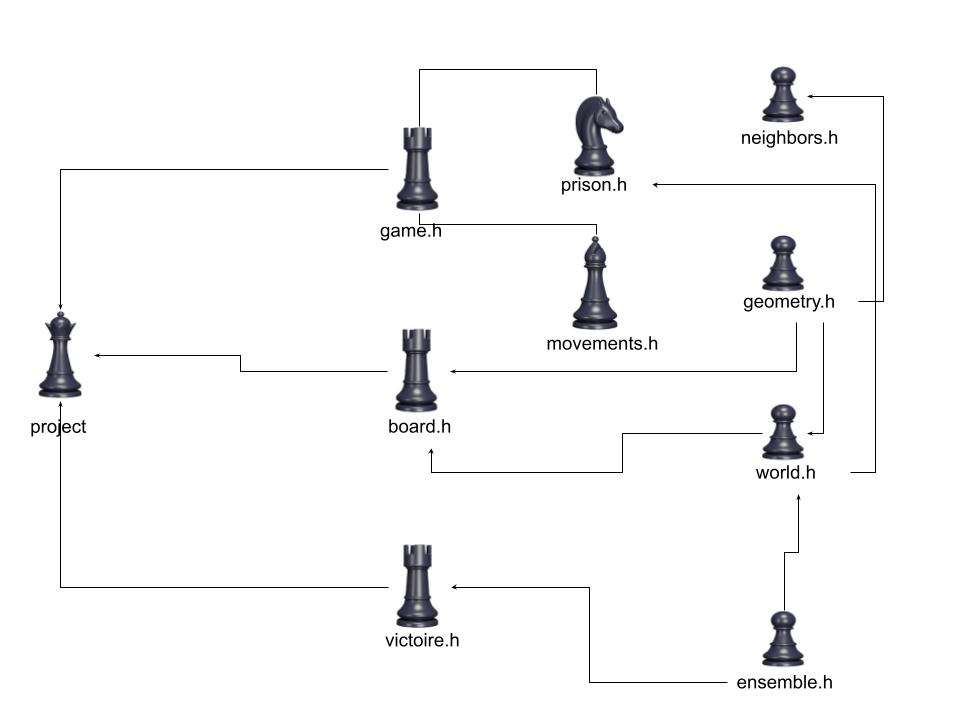
\includegraphics[scale=0.5]{Dessin sans titre.jpg} 

\end{center}

\section{INTRODUCTION}
\subsection{Problèmatique}
Mansuba est un jeu de plateau , ancêtre de Shtranj , qui a comme but mettre l’autre de joueur en situation de mat . 
Le but de notre projet sera de jouer une partie de jeu aléatoire, puis rendre l'algorithme de plus en plus flexible et général
et l'orienter finalement vers la victoire. 
\subsection{Hypothèse et démarches de validation}
Pour jouer une partie du jeu, il faut que le plateau de jeu soit définie au préalable. Le plateau de jeu \textit{board}  étant le binôme monde et relation. 
Le monde \textit{world} est l’ensemble des cases accessibles par les pions et dont les mouvements seront permis . Chaque case a désormais des cases voisines \textit{Neighbors} dans des directions précisé par \lstinline|enum dir_t|.
Le besoin 
La possibilité d’accès à ses voisins sera contrôlée par la relation de la partie et qui choisira parmis voisins ceux qui sont accessibles par mouvement direct.  
\section{Version initiale du jeu}
Dans cette partie le jeu a une configuration spécifique mais qui est plus simple à manipuler. Le jeu s’effectue sur une grille simple dans un monde a $\textcolor{purple}{\textsc{world\_size}} = \textcolor{purple}{\textsc{width}} \times \textcolor{purple}{\textsc{height}}$  case , que des pions simples (\lstinline|enum sort_t|) pour les joueurs ayant la couleur blanc et noir ()\lstinline|enum color_t|) . Cette configuration est surtout gouvernée par \textcolor{green}{\textit{geometry.h}}. \\
Pendant le développement du jeu 
Pour jouer une partie aléatoire on aura besoin de :
\subsection{Configurer le plateau de jeu}
\subsubsection{Partie monde}
La structure world est un tableau de pair couleur et type de pions qui inaccessible que par des fonctions de \textcolor{green}{\textit{world.h}}. On commence d’abord par initier un monde sans aucun pion à l’aide de la structure \lstinline|struct world_t* world_init();|. Cette fonction attribue à chaque case du tableau monde le pair \textcolor{purple}{\textsc{(no\_color , no\_sort)}}. Les fonctions de world.h permettront l’écriture et la lecture de la couleur et du type d’une case donné et seront utilisé fréquemment pour accéder au monde.  

\subsubsection{Partie relation}
La structure \lstinline|struct neighbors_t| prédéfinira les voisins de chaque indice donné . Les voisins seront un tableau dont le contenu pour un indice donné est un tableau de vecteur introduit par la structure \lstinline|struct vector_t| défini par l’indice du voisin et sa direction de taille \textcolor{purple}{\textsc{max\_neighbors}} . De la même façon que world, les fonctions qui donne accès au voisins sont \lstinline|struct neighbors_t get_neighbors(unsigned int idx)| qui cherche dans la structure des voisins l’élement d’indice rentré en paramètre et \lstinline|unsigned int get_neighbor(unsigned int idx, enum dir_t d)|qui aide à obtenir le voisin dans une direction donné par des opérations sur l’indice.\\ 

L’initialisation d’une relation modifie la liste des voisins pour qu’il puisse inclure que des voisins de certain directions donné. Avant d’initialiser une relation on pose dans la structure neighbors comme premier voisin pour chaque indice le pair \textcolor{purple}{\textsc{(uint\_max , no\_dir)}} et un (0,0) pour le reste. \textcolor{purple}{\textsc{uint\_max}} est définie dans \textcolor{green}{\textit{limits.h}}. La fonction add\_neighbor servira par suite à pousser \textcolor{purple}{\textsc{(uint\_max , no\_dir)}} et le remplacer par le pair indice du voisin et sa direction 
\subsection{Ensemble}
Cette structure \lstinline|struct ensemble|  permettra de construire des tableaux d’une taille donnée et simplifier leurs manipulations : lecture et écriture , comme le jeu a plusieurs collections à fournir : l’ensemble des positions des pions, la collection des mouvement possibles (qui sera le but de l’étape qui suit) ... . Elle contient comme attribut un entier qui donne la taille et un tableau d'indice qui sont le contenu de l'ensemble.
\subsection{Mouvements}
On a défini en plus une fonction qui sera utile pour le reste add\_position qui augmente la taille et remplace la position d’indice rentré en paramètre par sa valeur. 
Pour stocker les mouvements on fera appel à la structure ensemble . Les mouvement possibles dans la version de bases sont :  

    \textbf{\textcolor{magenta}{Déplacement simple}} : pour les relever il suffit d’utiliser la fonction get\_neighbors pour un indice donné . Ils seront stockés par la fonction \lstinline|void simple_moves( struct game_t game, struct ensemble* sm );|

    \textbf{\textcolor{magenta}{Saut simple}} : si le voisin dans une direction j est occupé, équivalent d’avoir la fonction get\_neighbor dans la direction j qui a un \textsc{sort} différent de \textcolor{purple}{\textsc{no\_sort}}, et le voisin du voisin dans la meme direction est libre ,  on peut se déplacer vers le voisin du voisin , si le monde le permet. Ils seront stockés par la fonction \lstinline|void simple_jumps(struct game_t game , struct ensemble* sj);|
    
    \textbf{\textcolor{magenta}{Saut multiple}} : s’agit d’une suite de saut simple . Cette fonction avait besoin d’une condition d’arrêt pour éviter de boucler infiniment sur les sauts simples autre que les deux voisins soient occupés. Pour cela il nous fallait une fonction qui vérifie l’existence d’un élément dans un ensemble donné \lstinline int place_visited(struct ensemble* ens, unsigned int place );|Elle renvoie un 0 si la place n’est pas encore mentionnée dans l’ensemble qui sera notre condition pour arrêter la recherche. Ils seront stockés par la fonction \lstinline|void multiple_jumps(struct game_t game , struct ensemble* mj )|

Ses fonctions prennent comme paramètre additionnel un ensemble. Il servira comme espace de stockage pour chacune des fonctions au lieu de retourner l’ensemble à la fin de chacune . En plus, la fonction \lstinline|void available_movements(struct game_t game, struct ensemble* am) |fera appel à toutes les fonctions de mouvement citée au-dessus et l’ensemble rentrer comme paramètre dans cette fonction sera le même rentrer dans tous les fonctions pour qu’on puisse stocker tous les mouvements dans un même ensemble.  
\subsection{Positions de départ et victoires}
Le monde étant inacessible par d’autre document autre que \textcolor{green}{\textit{world.h}}. On a utilisé les fonctions \lstinline|void world_set(struct world_t* b, unsigned int idx, enum color_t c)| et \lstinline|void world_set_sort(struct world_t* b, unsigned int idx, enum sort_t c)|pour donner à un monde initialisé vide des positions pour chacun des pions. Le nombre des pions étant \textcolor{purple}{\textsc{height}}.  

Il existe deux types de victoires. La victoire est dite simple si le joueur atteint une des positions de départ de l’autre joueur et complexe si le joueur les atteint tous. En tous cas, on aura besoin de garder la liste de positions de départ des deux joueurs et leurs faire rentrer en paramètre pour pouvoir comparer avec les positions actuelles de l’adversaire. En plus, pour la comparaison on pourra utiliser la fonction place\_visited. 

Le jeu s’arrête si on atteint une victoire, le choix du type étant aléatoire pendant la partie, ou si on atteint \textcolor{purple}{\textsc{max\_turns}}. 
\subsection{Boucle de jeu}
Avant d’obtenir la boucle de jeu finale il faudra définir des fonctions qui font des choix aléatoires sur tous les paramètres du jeu. 
Le choix du pion sera fait par \lstinline|void choose_random_piece_belonging_to(struct game_t* game) |qui retournera un indice. La fonction \lstinline| unsigned int choose_random_move_for_piece(struct game_t game)| va chercher entre les mouvements disponibles pour cet indice et va ensuite choisir un indice auquel le pion va bouger. La fonction \lstinline|void move_piece(struct game_t game, unsigned int dst)| agira sur le monde et échangera l’état de la case à l’indice initial avec celle de l’indice du mouvement. On choisira ainsi aléatoirement le premier joueur à commencer. 



\section{Amélioaration du jeu}

Dans cette partie on cherche à rendre le jeu de plus en plus générique pour qu'il nous offre plus de possibilités. La version initaile (2) est un peu basique car il contient le même type de pièces avec les mêmes déplacements.
Alors dans la suite on va essayer en premier temps de définir plusieurs types de pièces(Tour, Éléphant) avec de nouveau mouvements possibles(translation cardinal et saut semi-diagonal), avant de passer , et finalement ajouter la possibilité de capturer les pièces du joueur adversaire pour que la partie soit plus intéréssante et amusante.
\subsection{Mettons nous au pièces}
\subsubsection{Tour}


\subsubsection{Éléphant}


\subsection{grille}


\subsection{possibilité de capture}
\subsubsection{}

\end{document}